\chapter{Theorie}
\label{sec:Theo}
In dieser Bachelorarbeit wird untersucht, wie mithilfe von organischen Kristallen THz-Strahlung erzeugt wird. 
Dabei werden in diesem Kapitel die physikalischen Grundlagen für diese Erzeugung erläutert.
Zu Beginn wird in \autoref{sec:NLO} 
erklärt, wie die nichtlinearen Prozesse genutzt werden, um THz-Strahlung zu erzeugen und was diese auszeichnet. 
Danach wird in \autoref{sec:OR} erklärt, wie die THz-Strahlung im Kristall erzeugt wird. 
Dazu wird in \autoref{sec:PA} genauer erläutert, wie Phasenanpassung
die nutzbaren Kristalldicke begrenzen.
% Diese Kristalle, die zur Erzeugung von THz-Strahlung in der Bachelorarbeit genutzt wurden, 
% werden in \autoref{sec:ME} genauer beleuchtet. 
Zum Abschluss wird in \autoref{sec:TEOS} die Theorie hinter dem Messverfahren und der Signalverarbeitung des Aufbaus erklärt.



\section{Nichtlineare Optik}
\label{sec:NLO}
In der Optik sind die meisten Phänomene linearer Natur. 
Dies bedeutet, dass die elektrische Polarisation eines Mediums 
linear auf ein extern angelegtes elektrisches Feld $E$ antwortet.
Doch wenn das elektrische Feld eine 
Stärke von $\sim3\cdot10^{11}\,\unit{V/m}$ oder mehr erreicht, werden nichtlineare Beiträge wichtig. 
Eine solche Feldstärke ist nur mit der Nutzung von Lasern erreichbar, welche 
hier für diese Arbeit genutzt werden \cite{Butcher_Cotter_1990}. 
Die Nichtlinearität wird sichtbar, wenn ein Medium semiklassisch genähert wird und zuerst 
die lineare Lösung gezeigt wird. 
Das Medium wird genähert als ein positive Kern und ein daran durch eine Feder befestigtes Elektron. 
Dabei kann der positiver Kern als räumlich fest angenommen werden, da die 
Elektronen deutlich leichter als die Protonen sind.
Wenn an dieses System ein elektrisches Feld angelegt wird, kann 
dieses in erster Näherung als getriebener harmonischer Oszillator genähert werden. 
Es ergibt sich aufgrund der Coulomb-Wechselwirkung zwischen dem Elektron und dem $E$-Feld die Bewegungsgleichung 
\begin{equation}
    \label{eqn:bew}
    m\left(\frac{\text d^2x}{\text d t^2}+2\Gamma \frac{\text d x}{\text d t}+\Omega^2\cdot x-\left(\xi^{(2)}x^2+\xi^{(3)}x^3+\dotsb\right)\right)= -e E(t)
\end{equation}
für das Elektron.
Hier ist $m$ die Masse des Elektrons, $x$ die Auslenkung aus der Ruhelage, $\Gamma$ 
die Dämpfungskonstante, 
$\Omega$ die Eigenfrequenz des Systems und $\xi$ die anharmonischen Kraftterme.
Dabei werden im linearen Fall die anharmonischen Lösungen, $\xi^{(i)}=0\, \forall i \ge 2$, angemommen. 
%Genaueres dazu kann in \cite{Butcher_Cotter_1990} gelesen werden.
Dies ist der Unterschied zum nichtlinearen Ansatz, da dort die anharmonischen Teile 
nicht vernachlässigt werden können. 
Bildlich gesprochen wird in diesem Fall die Feder, die den positiven Kern und das Elektron 
miteinander verbindet, so weit auseinandergezogen, dass die Reaktion der Feder nicht mehr 
Linear ist.\\ 
Die Polarisation $P$ ist wiederum nicht so einfach im Federbild darstellbar. 
Die Polarisation beschreibt die Antwort des Mediums von einem 
eingehenden elektrischen Felds. 
Mathematisch beschrieben wird diese als $P(t)= -N\cdot e\cdot x(t)$, mit $N$ als Teilchendichte, 
$e$ als Ladung des Elektrons und $x(t)$ als Auslenkung des Elektrons aus der Ruhelage. 
Somit lässt sich mit der Lösung von \eqref{eqn:bew} im linearen, harmonischen Fall, die Polarisation 
\begin{equation}
    P =  \epsilon_0 \chi^{(1)}E  
\end{equation}
bestimmen.
Im nicht harmonischen, also nichtlinearen Fall ist dies aber nicht exakt zu bestimmen und 
eine Taylor-Reihen-Entwicklung wird angewendet. 
Dadurch ergibt sich
\begin{equation}
    \label{eqn:NLP}
    P_{i} = \epsilon_0 \left(\chi^{(1)}_{i,j}E_J+\chi^{(2)}_{i,j,k}E_j E_k+\chi^{(3)}_{i,j,k,l}E_j E_k E_l\dotsb\right)\, .
\end{equation}
Dort beschreibt $\chi^{(1)}$ die lineare Suszeptibilität und die folgenden $\chi^{(2)}_{i,j,k}$, $\chi^{(3)}_{i,j,k,l}$,
die nichtlinearen Suszeptibilitäten des Mediums \cite{Butcher_Cotter_1990}.
Das $\chi^{(2)}_{i,j,k}$ ist hierbei ein Tensor dritter Stufe und besitzt zusätzlich die Abhängigkeiten 
$i$, welche die Polarisation beschreibt, und $j$ und $k$ welche Komponenten des Feldes sind.
Die Anzahl der unabhängigen Komponenten lässt sich durch Kristall- und Permutationssymmetrien reduzieren.
Für den Prozess der optischen Gleichrichtung ist der $\chi^{(2)}_{i,j,k}$-Term entscheidend. 
Dabei ist wichtig, dass dieser Term in bestimmten Fällen wegfällt, 
zum Beispiel bei einem Medium, welches inversionssymmetrisch ist. \\
Das kann mithilfe der Inversionsoperation als Symmetrietransformation gezeigt werden \cite[Kap. 5.3.2]{Butcher_Cotter_1990}. 
Diese Symmetrieeigenschaft wird auch als Zentrosymmetrie bezeichnet, 
welche in nur 11 der 32 Kristallgruppen vorliegt und die somit nicht für die Generation von THz infrage kommen \cite{Jazbinsek2019}. 
Des Weiteren ist es von Vorteil, wenn die Polarisation im Frequenzbild betrachtet wird, um zum Beispiel die Differenzfrequenz zu nutzen. 
Dafür wird angenommen, dass sich das elektrische Feld $E$ aus mehreren Frequenzkomponenten 
zusammensetzt, also definiert ist durch
\begin{equation}
    \label{eqn:frq}
    E(t)=E_1e^{i\omega_1 t}+E_2e^{i\omega_2 t} + \text{c.c.}\ .
\end{equation}
Wird \eqref{eqn:frq} in \eqref{eqn:NLP} eingesetzt, so entstehen durch das Quadrieren
Terme bei neuen Frequenzen wie die zweiten Harmonischen $2\omega_1$ und $2\omega_2$, die
Summenfrequenz $\omega_1+\omega_2$ sowie die Differenzfrequenz $\omega_1-\omega_2$.
Die beiden letztgenannten Prozesse entstehen aus den Kreuztermen der beiden Felder,
wobei die Differenzfrequenz erst durch die Berücksichtigung des komplex konjugierten
Anteils auftritt.
Dies wird Drei-Wellen-Mischung genannt, da die zwei Eingangsfelder und das eine Ausgangsfeld betrachtet werden \cite{Boyd2023}. 
Beide Strahlen stammen jedoch aus demselben Laser und besitzen daher zunächhst identische Frequenzkomponenten.
Hierbei ist aber entscheidend, dass der Laser ein Ultrakurzpulslaser im fs-Bereich ist 
und durch die Zeit-Bandbreiten-Unschärfe $\symup{\Delta} t\cdot \symup{\Delta} \nu \ge \text{const.}$ 
eine große Frequenzbandbreite besitzt \cite{Boyd2023}. 
Somit besitzt dieser ultrakurze Puls eine große Bandbreite an Frequenzen, welche sich in 
der Drei-Wellen-Mischung mischen können. 
% Im anschließenden Kapitel wird gezeigt, wie mithilfe der Differenzfrequenzerzeugung 
% eines breitbandigen Pulses THz-Strahlung, durch die optische Gleichrichtung erzeugt werden kann.

% -----------------------978-3-030-73893-8 in Downloads über TDS Kapitel 37 Lesen

\section{Optische Gleichrichtung}
\label{sec:OR}
Die optische Gleichrichtung erzeugt die THz-Strahlung über den nichtlinearen Prozess der 
Differenzfrequenz. 
Dieser liegt vor, wenn die beiden elektromagnetischen Wellen, welche auf das 
Material treffen, 
hier zwei Teile des selben breitbandigen Nah-Infrarot-Pulses, 
eine sehr ähnliche Frequenz besitzen und, somit die Differenz 
$\omega = \omega_1 - \omega_2$ sehr klein ist und im THz-Bereich liegt. 
Für die Polarisation, bei der die beiden elektrischen Felder betrachtet werden, bedeutet das 
\begin{equation}
     P(\omega)=\epsilon_0\chi^{(2)}(\omega=\omega_1-\omega_2)E(\omega_1)E^*(\omega_2) \, .
\end{equation}
Diese Polarisation beschreibt die Bewegung der durch das Feld erzeugten Dipole, wobei diese 
Dipole wieder ein elektrisches Feld erzeugen. 
\begin{wrapfigure}[15]{r}{0.45\textwidth}
  \centering
  \vspace{-\intextsep}
  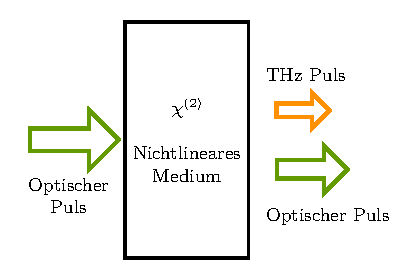
\includegraphics[width=\linewidth]{content/bilder/thz_erz.pdf}
  \caption{Grafische Darstellung der Erzeugung von THz-Strahlung, wobei nur ein kleiner 
         THz-Puls erzeugt wird und ein Großteil des optischen Pulses durch das Medium 
         hindurch dringt.}
  \label{fig:erz}
\end{wrapfigure}
Diese Polarisation wird von einem Teil der NIR-Welle erzeugt, aber nicht vollständig absorbiert, 
was in \autoref{fig:erz} anschaulich dargestellt ist. 
Berechnet wird das elektrische Feld, indem die Polarisation zuerst durch eine Fourier-Rücktransformation in die 
Zeitdomäne gebracht wird und anschließend durch die Maxwellgleichungen über die 
zweite Ableitung des erzeugten Feld berechnet werden \cite{Yu2022}. 
Somit ergibt sich für das elektrische Feld
\begin{equation}
    \label{eqn:ENL}
    E_\text{THz}\propto \frac{\partial^2P(t)}{\partial t^2}\, .
\end{equation}
Damit die an verschiedenen Stellen im Kristall erzeugte THz-Strahlung konstruktiv interferieren, 
muss vorher eine Phasenanpassung durchgeführt werden. Dies wird im Folgenden erklärt.
\section{Phasenanpassung und Kohärenzlänge}
\label{sec:PA}
Da der erzeugte THz-Puls eine unterschiedliche Phasengeschwindigkeit zu dem erzeugenden Pump-Puls besitzt, entsteht innerhalb des Kristalls Dispersion. 
Dadurch entsteht eine Phasenverschiebung zwischen dem Pumpstrahl und die erzeugte THz-Strahlung. 
Durch diese ist es möglich, dass destruktive Interferenz entsteht und die Intensität der Strahlung 
geringer ausfällt. 
Um zu gewährleisten, dass der erzeugte THz-Puls und der Pump-Puls dieselbe Phase haben, 
werden als erzeugendes Medium doppeltbrechende Kristalle verwendet. 
Diese haben entlang ihren Achsen verschiedene Brechungsindizes und erzeugt so eine unterschiedliche 
Phasenverschiebung. 
Um die Verschiebung anzupassen, kann der Kristall gedreht werden, wodurch die Phasen 
der beiden Felder angepasst werden. \\ \\
Entscheidend ist, dass das Kristallmaterial und die 
Wellenlänge des Pumpstrahls so gewählt werden, dass die Gruppengeschwindigkeit des 
Pumpstrahls möglichst nah an der Phasengeschwindigkeit des THz-Pulses ist. 
Innerhalb des Kristalls wird THz-Strahlung nur an einem Punkt, 
sondern entlang der gesamten Propagationsstrecke erzeugt. 
Unterscheiden sich Gruppengeschwindigkeit des Pumppulses und Phasengeschwindigkeit der THz-Welle, 
laufen die erzeugten Beiträge auseinander.
Ausschlaggebend sind die Brechungsindizes bei der Wellenlänge des Pumpstrahls $n_g^\text{NIR}$ 
und $n^\text{THz}$ bei der Wellenlänge von THz-Strahlung, zwischen denen  
\begin{equation}
    \label{eqn:brech}
    n_\text g^\text{NIR}(\lambda_\text{Pump})= n^\text{THz}(\lambda_\text{THz})
\end{equation}
gelten muss. In der Realität ist diese perfekte Anpassung aber nicht möglich und 
die Pulse laufen über längere Distanzen immer auseinander, wodurch der erzeugte Puls auch 
auseinanderläuft und so die Maxima und Minima verschwimmen. 
Wie weit ein Puls stabil bleibt, ist durch die Kohärenzlänge gegeben.
Diese Kohärenzlänge $l_\text{k}$ ist durch 
\begin{equation}
    \label{eqn:koh}
     l_\text{k}= \frac{c}{2\nu\cdot |n^\text{THz}(\nu_\text{THz})-n^\text{NIR}_\text{g}(\lambda_\text{Pump})| }
\end{equation}
gegeben \cite{brunner2014thz}.
Hierbei ist $c$ die Lichtgeschwindigkeit im Vakuum und $\nu$ die Frequenz der erzeugten THz-Strahlung.


\section{Elektrooptische Detektion und Signalverabeitung}
\label{sec:TEOS}
Die elektrooptische Detektion ist ein Messverfahren, mit welchem die generierte THz-Strahlung 
Zeitaufgelöst gemessen werden kann. 
Die Detektion startet im Detektionskristall, welcher ein nicht inversionssymmetrischer 
Kristall sein muss. In diesem werden der THz-Strahl und der Detektions-Strahl räumlich und zeitlich überlappt. 
Durch das elektrische Feld im Kristall tritt der Pockels-Effekt auf.
Dieser ist ein nichtlinearer Prozess zweiter Ordnung und wird durch \autoref{eqn:NLP} beschrieben. 
Durch diesen wird der Kristall doppeltbrechend,   
die Stärke der Doppelbrechung ist proportional zu der elektrischen Feldstärke der THz-Strahlung. 
Durch die Doppelbrechung wird die Polarisation von dem Detektionsstrahl gedreht. 
Somit wird aus der linearen Polarisation des Lichts vom Laser eine elliptische Polarisation \cite{zheng2023probing}. 
Der THz-Puls ist hierbei mehrere ps lang und der Detektionspuls nur $\approx\SI{30}{fs}$. Dadurch kann der deutlich kürzere Detektionspuls 
den längeren THz-Puls abtasten.
\autoref{fig:EOS} zeigt schematisch den Aufbau einer elektrooptischen Detektion, wobei sich die Strahlen von links nach rechts bewegen. 
Die Pfeile zeigen die Polarisation des Pulses an verschiedenen Stellen.
\begin{figure}
    \centering
    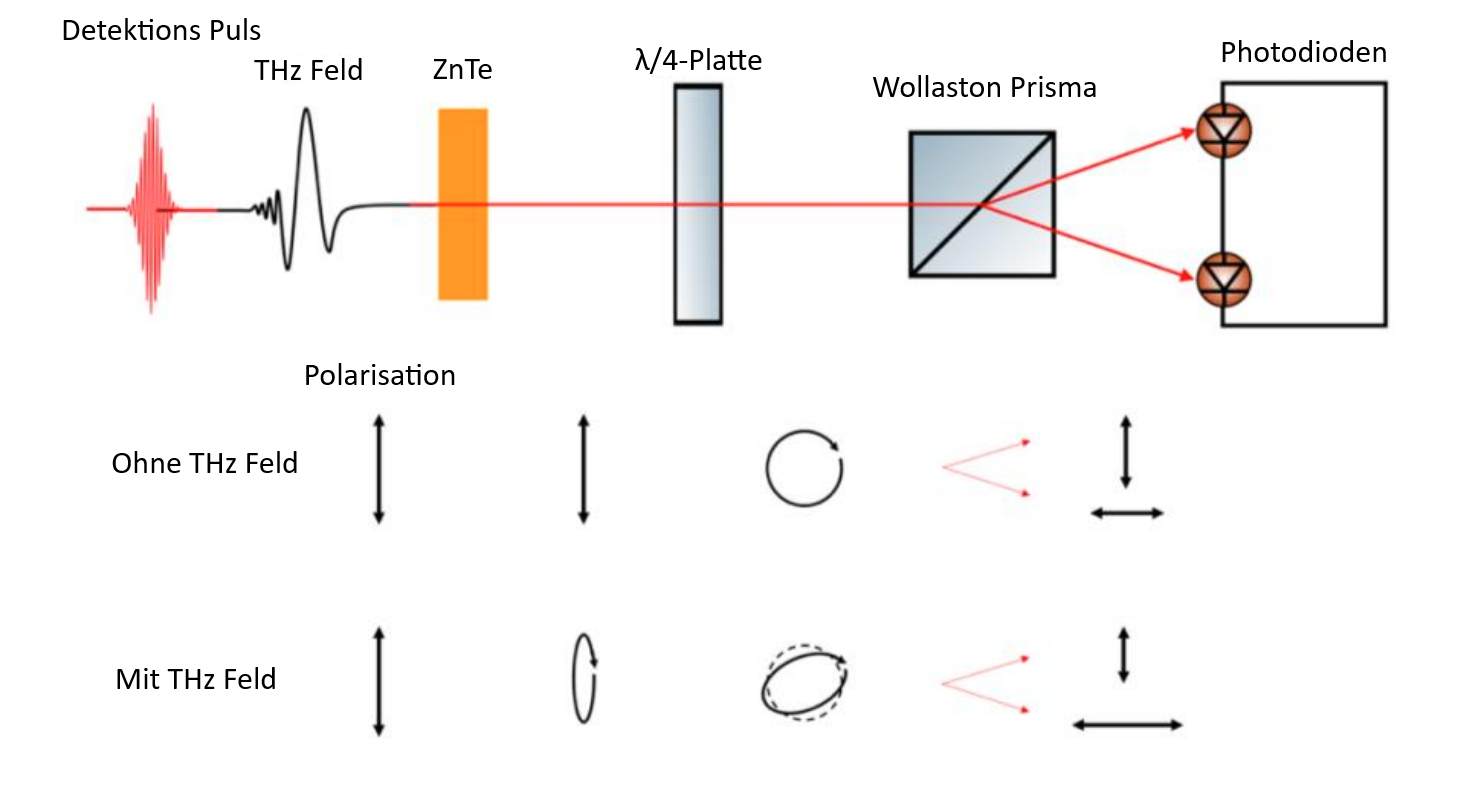
\includegraphics[width=0.8\textwidth]{content/bilder/eos_p.png}
    \caption{Schematischer Aufbau der elektrooptischen Detektion, Grafik entnommen aus \cite{zheng2023probing}.
     Oben ist der Pulsverlauf von links nach rechts zu sehen, wobei der Detektionspuls und der Thz-Puls gleichzeitig durch den Aufbau gehen. 
     Der Aufbau besteht in dieser Reihenfolge aus einem ZnTe-Kristall, einer $\lambda/4$-Platte, einem Wollaston-Prisma und zwei Photodioden. 
     Unter dem Aufbau ist schematisch die Polarisation des Pulses einmal mit und einmal ohne den THz-Puls zu sehen und wie diese sich über den Aufbau verhält.}
    \label{fig:EOS}
\end{figure}
Anschließend durchläuft der im ZnTe-Kristall elliptisch polarisierte Detektionsstrahl eine
$\lambda/4$-Platte. Diese führt zwischen der ordentlichen und der außerordentlichen
Polarisationskomponente eine Phasenverzögerung von \SI{90}{\degree} ein. Steht die
Polarisation eines linear polarisierten Strahls unter \SI{45}{\degree} zur optischen Achse
der Platte, so werden beide Komponenten mit gleicher Amplitude angeregt und der Strahl
verlässt die Platte zirkular polarisiert. Dieser Winkel wird durch Drehen der
$\lambda/4$-Platte eingestellt.
Ohne THz-Feld ist der Detektionsstrahl hinter der $\lambda/4$-Platte somit zirkular
polarisiert. 
Während unter Einfluss des THz-Feldes ein elliptisch polarisierter Strahl entsteht.
Anschließend trifft dieser Strahl auf ein Wollaston-Prisma, 
dieser unterteilt die horizontale und vertikale Polarisation räumlich. 
Diese abgelenkten Strahlen werden auf die Photodioden gelenkt.
Wenn kein THz-Feld auf den Detektionskristall trifft, ist die Polarisation vor dem 
Wollaston-Prisma ein perfekter Kreis und beide dieser Polarisationsanteile sind identisch. 
Jedoch hat das THz-Feld eine Rotation der Polarisation ausgelöst und die Anteile 
sind nicht mehr identisch. 
Somit ist die Intensität auf den Photodioden nicht gleich. 
Der Intensitätsunterschied, den die Photodioden messen, ist proportional zur Feldstärke der 
THz-Strahlung. 
Diese Proportionalität ist, bei optimaler Orientierung des Kristalls, gegeben durch
\begin{equation}
    \symup{\Delta} I  =  \frac{ \pi}{2\cdot\lambda_0\cdot n_0}I_0 Ld_\text{THz}E_\text{THz}\propto E_\text{THz}\ .
\end{equation}
Hierbei ist $\symup{\Delta}I$ die gemessene Intensitätsdifferenz an den Photodioden, $I_0$ ist die Intensität des Detektionsstrahls 
vor dem Detektionskristall, $\lambda_0$ ist die Wellenlänge des Detektionsstrahls, $L$ die Dicke des Detektionskristalls, 
$n_0$ der Brechungsindex des Detektionskristalls bei der Wellenlänge $\lambda_0$, $d_\text{THz}$ ist der nichtlineare Koeffizient des 
ZnTe für die Richtung, durch welche der Strahl auf den ZnTe-Kristall trifft und $E_\text{THz}$ ist die elektrische Feldstärke des 
THz-Strahls an der Stelle, and der er mit dem Detektionsstrahl überlappt \cite{Planken2001}.
Hierbei ist die entscheidende Erkenntnis, dass der gemessene Stromunterschied an den Photodioden proportional zu dem 
THz-Feld und dadurch auch zu dem nichtlinearen Koeffizienten des Kristalls.

% \section{Elektro-Optische-Detektion und Signalverabeitung}
% \label{sec:EOS}

% Durch den Pockelseffekt wird wie in \autoref{sec:TEOS} beschrieben die Polarisation gedreht und die änderung 
% wird über die Elektro Optische Detektion gemessen.
Des Weiteren gibt es im gesamten Aufbau verschiedene Rauschquellen wie das Intensitätsrauschen des Lasers, 
Streulicht oder elektronisches Rauschen der elektrischen Komponenten der Detektionsbauteile.
Der THz-Strahl wird durch den Chopper mit der halben Repetitionsrate des Lasers moduliert. 
Im Lock-In-Verstärker wird das Photodiodensignal ausgelesen. 
Somit wird immer ein Puls mit und ohne THz-Strahlung detektiert. 
Im Lock-In wird die Demodulationsfrequenz mit dem Signal der Photodioden multipliziert. 
Dadurch landet der Signalanteil, welcher dieselbe Frequenz wie das Referenzsignal besitzt 
bei ungefähr $\SI{0}{Hz}$. 
Die restlichen Signale, welche nicht auf der Modulationsfrequenz liegen, werden auf andere Frequenzen 
verschoben. 
Anschließend wird das Produkt der Signale durch einen Tiefpassfilter geleitet, 
dieser lässt nur ein sehr schmales Frequenzband um $\SI{0}{Hz}$ passieren. 
Der Tiefpassfilter integriert über eine Zeit $\tau$, welche auch Zeitkonstante genannt wird. In dieser Bachelorarbeit 
werden verschiedene Zeitkonstanten, welche mehrere Größenordnungen über der Periodendauer des Lasers liegen, genutzt. 
Die Proportionalität zwischen Rauschen und Zeitkonstante wird beschrieben durch 
\begin{equation}
    \label{eqn:tc}
    U_\text{Rauschen} \approx \frac{A}{\sqrt{\tau}}\,.
\end{equation} 
$U_\text{Rauschen}$ ist die vom Lock-in-Verstärker ausgegebene Rauschspannung. 
$A$ ist hierbei eine Konstante, 
welche die Rauschamplitude beschreibt \cite{zhinst_lockin_whitepaper}.
Zusätzlich ist das Rauschen invers proportional mit $\propto \frac 1 f$ zur Modulationsfrequenz \cite{10.1063/1.5047659}. 
In dieser Bachelorarbeit wird eine Modulationsfrequenz von \SI{1500}{HZ}, was der halben Repetitionsrate des Lasers entspricht, genutzt, 
welche die größtmögliche fundamentale der Wiederholrate der Laser-Pulse entspricht.





\chapter{Materialeigenschaften}
\label{sec:ME}

Wie in dem vorangegangenen Kapitel beschrieben, müssen die Materialien verschiedene Eigenschaften besitzen um 
THz Effektiv zu erzeugen. 
In dieser Bachelorarbeit werden ZnTe, OH1 und BNA genutzt und im folgenden kurz vorgestellt.

% Für die THz-Erzeugung sind spezielle Eigenschaften wie das Nichtvorhandensein einer Zentrosymmetrie 
% entscheidend. 
% Deshalb wurden die Materialien sehr bedacht gewählt. Die wichtigen Eigenschaften von diesen 
% werden im Folgenden beschrieben.
\section{Zinktellurid}
Zinktellurid, ist ein anorganischen Kristall, welcher in dieser Arbeit zur THz Generation und Detektion genutzt wird. 
Die Kristallstruktur von ZnTe ist in \autoref{fig:ZnTe} zu sehen, wobei Zink Orange und Tellur Blau gekennzeichnet ist. 
\begin{wrapfigure}[18]{r}{0.45\textwidth}
  \centering
  \vspace{-\intextsep}
  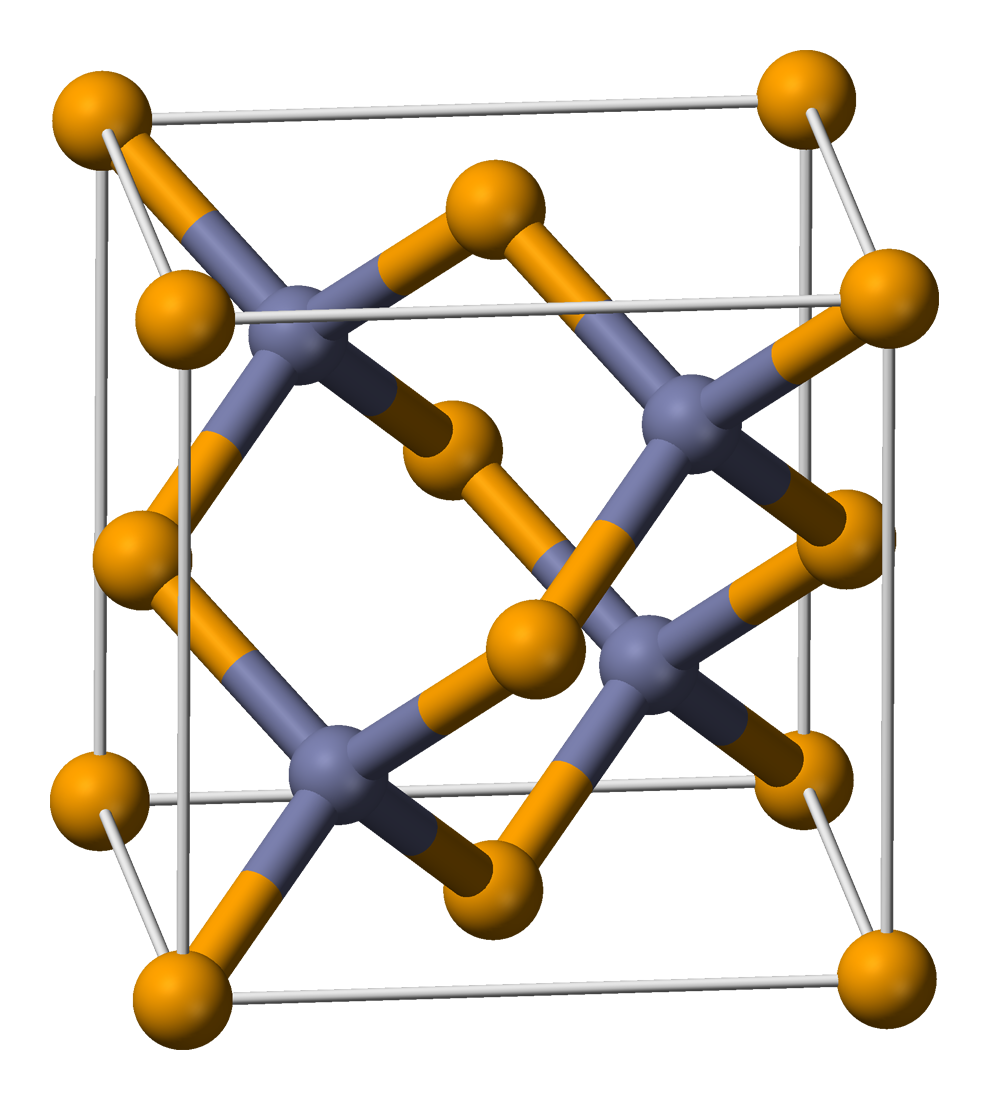
\includegraphics[width=\linewidth]{content/bilder/ZnTe.png}
  \caption{Grafische Darstellung der Gitterstruktur von ZnTe. 
  Wobei Zink Orange und Tellur Blau gekennzeichnet ist \cite{enwiki:1327029761}.}
  \label{fig:ZnTe}
\end{wrapfigure}
Die Gitterkonstanten von ZnTe betragen $a = b = c = \SI{6.101}{\angstrom}$. Der Kristall gehört zu der Raumgruppe 
F43m. 
und ist <110> orientiert \cite{Brach}. 
Dazu ist der nicht lineare Koeffizient bei $\SI{800}{nm}$-Strahlung $d_{\text{THz}}= \SI{59.9}{pm/V}$ \cite{Planken2001}.
Die Brechungsindizes  betragen $n_\text{THz}\approx \SI{3.276}{}$ bei 
$ \nu^*\approx \SI{2.43}{THz}$ \cite{tripathi2013accurate}und $n_\text{NIR}^\text{phase}\approx \SI{3.239}{}$ bei $\lambda^*\approx \SI{800}{nm}$ \cite{Planken2001}. 
Diese hier angenommene Wellenlänge ist wiederum nicht exakt die des $\SI{808}{nm}$-Lasers, welcher in diesem Aufbau 
genutzt wird. 
Deshalb werden in der Realität die Werte minimal abweichen.
Mit diesen Werten berechnet sich die Kohärenzlänge zu
$l_\text{k}\approx \SI{3}{mm}$.
Die transversale Phonenresonanzfrequenz ist $\Omega_\text{TO}/2\pi=\SI{5.32}{THz}$. 
Nahe dieser Frequenz absorbieren die Phonen einen großen Teil der Leistung und die THz-Generation 
ist deutlich geschwächt \cite{Tomasino}.
% Zusammenfassend ist ZnTe aber ein sehr guter THz-Erzeuger, da das Erzeugungsspektrum selbst bei nicht 
% Perfekter Phasenanpassungsfrequnz sehr gut für die Thz-Generation ist.
\section{OH1}
\label{sec:MOH1}
Als erster Organischer Kristall zur THz Generation dient,  2-(3-(4-
hydroxystyryl)-5,5-dimethylcyclohex-2-enylidene)malononitrile, kurz OH1. 
\begin{wrapfigure}[11]{r}{0.45\textwidth}
  \centering
  \vspace{-\intextsep}
  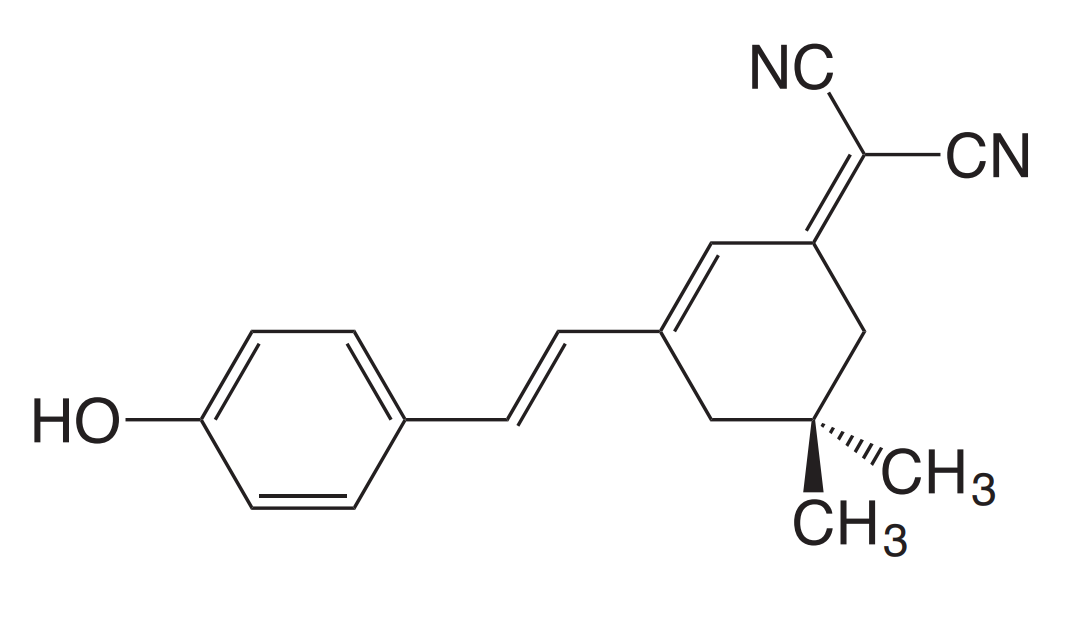
\includegraphics[width=\linewidth]{content/bilder/OH1_ch.png}
  \caption{Grafische Darstellung der Chemischen Struktur von OH1 \cite{brunner2008hydrogen}.}
  \label{fig:OH1_ch}
\end{wrapfigure}
Der Kristall gehhört der Raumgruppe Pna$2_1$ und der Punktgruppe mm2 an. 
Dazu hat der Kristall den Winkel $\theta_kz = 28°$ zwischen Ladungstransferachse und Polarer Achse c.
Die Chemische Struktur ist in \autoref{fig:OH1_ch} zu sehen.
Für den Nichtlinearen Koeffizient sind nur werte mit deutlich höheren Wellenlängen des Pumplasers vorhanden. 
Das liegt daran, da OH1 explizit mit einer höheren effizienz in dem Bereich um $\SI{1300}{\nano\meter}$ optimiert ist. 
Für einenen Pumplaser mit der Zentralwellenlänge von $\SI{1300}{\nano\meter}$ liegt der Nichtlineare Koeffizient bei $d_\text{THz}\approx\SI{280}{\pico\meter\per\volt}$.
Dieser Wert ist aber kritisch zu betrachten, da der genutzte Pumplaser bei einer Zentralwellenlänge von $\SI{808}{\nano\meter}$ liegt un somit 
sehr weit von dem referenzwert entfernt ist. 
In \cite{Jazbinsek2019} lässt sich wiederum der nichhtlinearel Graphisch zu $d_\text{THz}\approx \SI{490}{\pico\meter\per\volt}$
Die Brechungsindizes betragen gemäß \eqref{eqn:brech} $n^*_\text{g}=n^*_\text{THz}\approx \SI{2.3}{}$ bei 
$ \nu^*\approx \SI{1}{THz}$ und $\lambda^*\approx \SI{1300}{nm}$ \cite{Jazbinsek2019}.
Die Kohährenzlänge liegt bei $l_\text{k}\approx \SI{0.4}{\milli\meter}$ bei einer Pumpwellenlänge von $\SI{808}{\nano\meter}$ 
Dazu wird aber in \cite{Mansourzadeh2023} explizit beschrieben, dass bei Pumpwellenlänge unter $\SI{1100}{\nano\meter}$ keine Phasenanpassung möglich ist 
und somit die Kohährenzlänge niedriger als bei ZnTe ausfällt.
%und einer erzeugten THz frequenz von $f_\text{THz}\approx\SI{2}{\tera\hertz}$ \cite{Mansourzadeh2023}.
Die stärkste Phonenresonanzfrequenz liegt oberhalb der $\SI{10}{\tera\hertz}$ und bei $\SI{3}{\tera\hertz}$ und $\SI{4.5}{\tera\hertz}$ liegen 
zwei weitere \cite{Jazbinsek2019}.
Dort ist durch die Aborption eine geschwächte generation zu erwarten.

\section{BNA}

Als zweiten organischen Kristall für die THz-erzeugung wurde N-Benzyl-2-methyl-4-nitroaniline oder kurz BNA gewählt. 
Dieser wird der Raumgruppe Pna2 und der Punktgruppe mm2 zugeordnet. 
Der Winkel zsichen der Ladungstransferachse und der Polaren Achse beträgt $\theta k z = 33°$ \cite{Jazbinsek2019}. 
Der nichtlineare Koeffizient liegt bei $d_\text{Thz}=\SI{234}{\pico\meter\per\volt}$, wobei dieser bei einer Pump 
Wellenlänge von $\SI{1064}{\nano\meter}$ gemessen wurde und somit nicht vollständig auf den hier genutzten aufbau mit einer 
Pumpwellenlänge von $\SI{808}{\nano\meter}$ anwendbar ist. 
Der gruppen Brechungsindix bei der Pumpwellenänge beträgt $n_\text g^\text{NIR}\approx \SI{1.9}{}$ und der Phasen Brechungsindex bei der 
erzeugten THz-Strahlung, hier bei einem Peak von $\SI{1}{\tera\hertz}$, beträgt $n_\text{THz}\approx\SI{2.05}{}$ \cite{Mansourzadeh2023}. 
Die Kohährenzlänge sich Grafische in \cite{miyamoto2009optimized} zu $\l_\text{k}\approx \SI{0.4}{\milli\meter}$ bestimmen. 


